
The dynamic viscosity of a fluid is a function of fluid composition and temperature and typically has a weak dependence on pressure. In some applications, particularly those that involve large variations in temperature, viscosity can vary significantly in space and over time. Variations in viscosity, in turn, can affect groundwater flow by changing the hydraulic conductivity, which is inversely proportional to viscosity. In the original release of \mf, variations in viscosity and their effects on hydraulic conductivity were not taken into account. The \mf Viscosity (VSC) Package allows viscosity to vary as a function of solute concentrations and fluid temperature and accounts for the effect of variable viscosity on hydraulic conductivity in the Node-Property Flow (NPF) Package and in stress packages that involve head-dependent groundwater flow. Temperature-dependent viscosity has been implemented in other groundwater modeling codes, including HST3D \citep{kipp1987}, VS2DH \citep{healy1996}, SUTRA-MS \citep{hughes2004}, and SEAWAT Version 4 \citep{langevin2008seawat}. Like these other codes, the VSC Package does not account for the dependence of viscosity on pressure, which is negligible in most applications.

For cases in which the rate of groundwater flow is proportional to the head gradient in the direction of flow, as in an isotropic porous medium, the flow between two adjacent locations can be approximated using a one-dimensional form of Darcy's Law \citep[equation 4-15]{modflow6gwf}:

\begin{equation}
\label{eqn:modflow6gwf-4-15}
Q = C \left( h_{1} - h_{2} \right),
\end{equation}

\noindent where $h_{1}$ and $h_{2}$ are the hydraulic heads at locations 1 and 2, respectively, $Q$ is the flow from location 1 to location 2, and $C$ is a hydraulic conductance defined by~\citep[equation 4-14]{modflow6gwf}:

\begin{equation}
\label{eqn:modflowgwf-4-14}
C = \frac{K A} {L_{1,2}},
\end{equation}

\noindent where $K$ is the hydraulic conductivity of the porous medium that connects the two locations, $A$ is the cross-sectional area perpendicular to flow, and $L_{1,2}$ is the distance between two locations. A form of equation~\ref{eqn:modflow6gwf-4-15} is used in the \mf ``conductance-based'' formulation for flow between two adjacent model cells \citep{modflow6gwf}. In that case, the conductance is based on an effective hydraulic conductivity between the two cells, the area of the cell-cell interface, and the distance between the cell centers. A form of equation~\ref{eqn:modflow6gwf-4-15} is also used in \mf stress packages in which the flow into or out of the model at a model boundary is head-dependent. For example, in the General-Head Boundary (GHB) Package, flow between an external source and a groundwater model cell is proportional to the difference between the head assigned to the external source and the simulated head in the cell, and the conductance is representative of the material between the external source and the cell center.

Because hydraulic conductivity is inversely proportional to viscosity, the conductivity $K$ for a simulated fluid composition and temperature is related to the conductivity $K_{0}$ for some reference composition and temperature by

\begin{equation}
\label{eqn:conductivity-ratio}
K = \frac{\mu_{0}}{\mu} K_{0}.
\end{equation}

\noindent It follows from equation~\ref{eqn:modflowgwf-4-14} that the conductance $C$ for a simulated fluid composition and temperature is related to the conductance $C_{0}$ for the reference composition and temperature by

\begin{equation}
\label{eqn:conductance-ratio}
C = \frac{\mu_{0}}{\mu} C_{0},
\end{equation}

\noindent where $\mu$ and $\mu_{0}$ are the viscosities at the simulated and reference conditions, respectively. The VSC Package uses equations~\ref{eqn:conductivity-ratio} and~\ref{eqn:conductance-ratio} to update hydraulic conductivities and conductances to account for changes in solute concentrations and temperature during a flow and transport simulation based on the Groundwater Flow (GWF) and Groundwater Transport (GWT) Models. The GWT Model is designed to simulate solute transport but can be used to simulate heat transport in some applications by appropriately scaling the input parameters to render the solute-transport equation mathematically equivalent to the heat-transport equation \citep{zheng2010supplemental}. In such cases, the ``solute concentration'' calculated by a GWT-based heat-transport model can by identified in the VSC Package input file as representing temperature. Although the VSC Package allows viscosity to vary with solute concentration, variations in viscosity are typically most significant in heat-transport applications.

\subsection{Dependence of Viscosity on Concentration and Temperature} \label{sec:fluidvsc}

The VSC Package calculates viscosity as a function of concentration and temperature using the following equation \citep[equation 17]{langevin2008seawat}:

\begin{equation}
\label{eqn:viscfunc}
\mu = \mu_T \left ( T \right ) + \sum_{k=1}^{NS} \frac{\partial \mu} {\partial C^k} \left ( C^k - C_{0}^k \right ) 
\end{equation}

\noindent where $NS$ is the number of chemical species (solutes) whose concentrations affect viscosity, $C^k$ and $C_{0}^k$ are the simulated and user-specified reference concentrations of species $k$, respectively, and $\partial \mu / \partial C^k$ is the user-specified rate at which viscosity changes linearly with the concentration of species $k$. (Symbols $C^k$ and $C_{0}^k$ are not to be confused with the symbols for conducance, $C$ and $C_0$, introduced earlier.) When all concentrations are equal to their reference values, the viscosity is equal to $\mu_T \left ( T \right )$, which embodies the dependence of viscosity on temperature according to

\begin{align}
	\label{eqn:viscT}
	 \mu_T \left ( T \right ) = \begin{dcases}
		\mu_{0} + \frac{\partial \mu} {\partial T} \left ( T - T_{0}\right ) & linear \\
		\mu_{0} A_2^{\frac{A_3 \left ( T_0 - T \right )} {\left ( T + A_4 \right ) \left ( T_0 + A_4 \right ) }} & nonlinear
	\end{dcases} .
\end{align}

\noindent where $T$ and $T_{0}$ are the simulated and user-specified reference temperature, respectively, and $\mu_{0}$ is the user-specified reference viscosity. The reference viscosity is commonly set to 0.001 kg~m$^{-1}$~s$^{-1}$, which is representative of freshwater at a reference temperature of 20$^{\circ}$C \citep[Table 11.1]{maidment1993}. When $T$ equals $T_{0}$, or if temperature is not designated by the user as affecting viscosity, $\mu_T \left ( T \right )$ equals $\mu_{0}$. Equation~\ref{eqn:viscT} includes both linear and nonlinear variation of viscosity with temperature. Linear variation is the default, in which case $\partial \mu / \partial T$ is the user-specified rate at which viscosity changes linearly with temperature. Nonlinear variation is a user-selectable option, in which case the variation of viscosity from the reference value is determined by user-specified parameters $A_2$, $A_3$, and $A_4$. The nonlinear option in equation~\ref{eqn:viscT} is mathematically equivalent to one of the options available in SEAWAT Version 4 \citep[equation 18]{langevin2002seawat} but is written in a form that explicitly sets $\mu_T \left ( T \right )$ equal to $\mu_{0}$ when $T$ equals $T_{0}$. Setting $\mu_0$, $A_2$, $A_3$, and $A_4$ to 0.001002 kg~m$^{-1}$~s$^{-1}$, 10.0, 248.37, and 133.15, respectively, and rounding the lead coefficient to one decimal place gives the temperature dependence of viscosity used in SUTRA \citep{voss1984sutra} and SUTRA-MS \citep{hughes2004}. VS2DH \citep{healy1996} also calculate the temperature dependence of viscosity using functions that are, respectively, mathematically equivalent to and a special case of equation~\ref{eqn:viscT}.

Over the temperature range $0-40^{\circ}$C, the viscosity of freshwater varies between approximately 0.0007 and 0.00175 kg~m$^{-1}$~s$^{-1}$, as indicated by the nonlinear (blue) curve in figure~\ref{fig:viscosityrelation}. The black line in figure~\ref{fig:viscosityrelation} depicts a linear approximation that coincides with the nonlinear curve at the reference temperature and viscosity, $\left ( T_0, \mu_0 \right ) = \left(\right.$20$^{\circ}$C, 0.001 kg~m$^{-1}$~s$^{-1}\left.\right)$.

\begin{figure}
	\begin{center}
	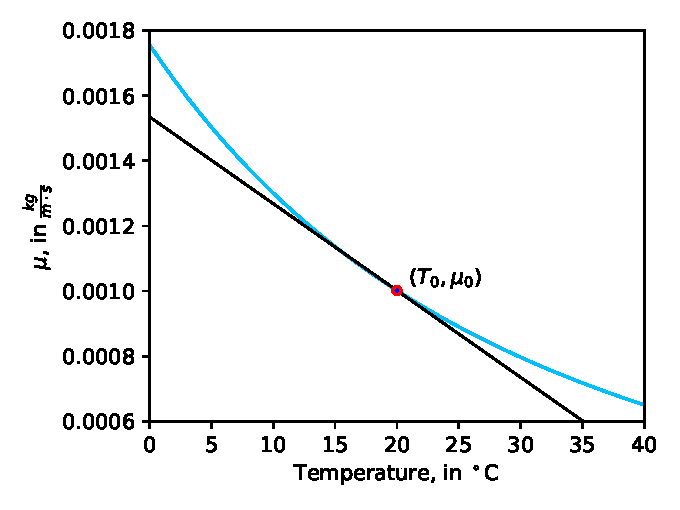
\includegraphics{./Figures/VSCnonlinear.pdf}
	\caption[Graph showing the nonlinear response in the viscosity as temperature changes]{Nonlinear dependence of viscosity on temperature (blue curve) that is representative of freshwater over the temperature range $0-40^{\circ}$C, and a linear approximation (black curve) that has the same value $\left ( \mu_0 \right )$ and slope at the reference temperature $\left ( T_0 \right )$.  The blue curve is generated using 0.001002 kg~m$^{-1}$~s$^{-1}$,10.0, 248.37, and 133.15 for $\mu_0$, $A_2$, $A_3$, and $A_4$, respectively}
	\label{fig:viscosityrelation}
	\end{center}
\end{figure}

\subsection{Accounting for Variable Viscosity in Flows Between Cells} \label{sec:gwfvsc}

The VSC Package uses concentrations and temperatures calculated for each cell by a GWT model on the previous time step or outer solution iteration to calculate viscosities for the current time step. These viscosities are used to adjust cell hydraulic conductivity values in the NPF Package using equation~\ref{eqn:conductivity-ratio}. The reference values of conductivity are the values specified by the user in the NPF Package and, optionally, the Time-Varying Conductivity (TVK) Package (Chapter 6 of this document). The conductivity adjustment is performed after the user-specified conductivities are read in but before conductivity values are passed to program units that use cell conductivities to formulate expressions for flow between cells, which include the ``conductance-based'' formulation for flow and the XT3D capability \citep{modflow6xt3d}. If the VSC Package is not active, cell conductivities are not adjusted for variable viscosity, and the user-specified values are used.

\subsection{Accounting for Variable Viscosity in Boundary Flows} \label{sec:gwfvsc}

The VSC Package uses concentrations and temperatures calculated for each cell by a GWT model on the previous time step or outer solution iteration in calculating viscosities for the current time step. These viscosities are used to adjust hydraulic conductances, using equation~\ref{eqn:conductance-ratio}, in stress packages that involve head-dependent boundary flows, which include the River (RIV), General-Head Boundary (GHB), Drain (DRN), Streamflow Routing (SFR), Lake (LAK), and Multi-Aquifer Well (MAW) Packages \citep{modflow6gwf}. For a boundary flow out of the model, the viscosity is based on the simulated concentration or temperature in the cell from which the boundary flow originates. For a boundary flow into the model, the viscosity is based on the concentration or temperature of the water entering the cell from the boundary. The reference values of conductance are the values normally set or calculated by the stress package based on user input. The conductance adjustment is performed after the stress package completes its normal conductance calculation but before the conductance value is used to formulate the expression for the boundary flow. If the VSC Package is not active, stress-package conductances are not adjusted for variable viscosity.

